\documentclass{acm_sen_article}


\usepackage{color}
% correct bad hyphenation here
\hyphenation{op-tical net-works semi-conduc-tor}
%\renewcommand{\baselinestretch}{0.93}

\begin{document}
%
% paper title
% Titles are generally capitalized except for words such as a, an, and, as,
% at, but, by, for, in, nor, of, on, or, the, to and up, which are usually
% not capitalized unless they are the first or last word of the title.
% Linebreaks \\ can be used within to get better formatting as desired.
% Do not put math or special symbols in the title.
\title{Automated Verification and Synthesis of Embedded Systems: Advances and Challenges}


% author names and affiliations
% use a multiple column layout for up to three different
% affiliations
\author{Lucas C. Cordeiro \\
Department of Computer Science\\
University of Oxford, UK\\
Email: lucas.cordeiro@cs.ox.ac.uk
\and
Eddie B. de Lima Filho \\
Science, Technology, and Innovation Center\\ for the Industrial Pole of Manaus, Brazil \\
Email: eddie@ctpim.org.br}
%\IEEEauthorblockN{Homer Simpson}
%\IEEEauthorblockA{Twentieth Century Fox\\
%Springfield, USA\\
%Email: homer@thesimpsons.com}
%\and
%\IEEEauthorblockN{James Kirk\\ and Montgomery Scott}
%\IEEEauthorblockA{Starfleet Academy\\
%San Francisco, California 96678--2391\\
%Telephone: (800) 555--1212\\
%Fax: (888) 555--1212}}

% conference papers do not typically use \thanks and this command
% is locked out in conference mode. If really needed, such as for
% the acknowledgment of grants, issue a \IEEEoverridecommandlockouts
% after \documentclass

% for over three affiliations, or if they all won't fit within the width
% of the page, use this alternative format:
% 
%\author{\IEEEauthorblockN{Michael Shell\IEEEauthorrefmark{1},
%Homer Simpson\IEEEauthorrefmark{2},
%James Kirk\IEEEauthorrefmark{3}, 
%Montgomery Scott\IEEEauthorrefmark{3} and
%Eldon Tyrell\IEEEauthorrefmark{4}}
%\IEEEauthorblockA{\IEEEauthorrefmark{1}School of Electrical and Computer Engineering\\
%Georgia Institute of Technology,
%Atlanta, Georgia 30332--0250\\ Email: see http://www.michaelshell.org/contact.html}
%\IEEEauthorblockA{\IEEEauthorrefmark{2}Twentieth Century Fox, Springfield, USA\\
%Email: homer@thesimpsons.com}
%\IEEEauthorblockA{\IEEEauthorrefmark{3}Starfleet Academy, San Francisco, California 96678-2391\\
%Telephone: (800) 555--1212, Fax: (888) 555--1212}
%\IEEEauthorblockA{\IEEEauthorrefmark{4}Tyrell Inc., 123 Replicant Street, Los Angeles, California 90210--4321}}



% make the title area
\maketitle

% As a general rule, do not put math, special symbols or citations
% in the abstract
\begin{abstract}
The dependency on the correct operation of embedded systems is rapidly growing, mainly due to their wide range of applications, such as micro-grids, automotive device control, health care, surveillance, mobile devices, telecommunications, and consumer electronics. Their structures are becoming more and more complex and now require multi-core processors with scalable shared memory and sophisticated software modules, in order to meet increasing computational power and flexibility demands. As a consequence, reliability of embedded (distributed) software becomes a key issue during system development, which must be carefully addressed and assured. Normally, state-of-the-art verification methodologies for embedded systems generate test vectors (with constraints) and use assertion-based verification and high-level processor models, during simulation. Nonetheless, other additional challenges have been raised: the need for meeting time and energy constraints, handling concurrent software, dealing with platform restrictions, evaluating implementation-structure choices, validating operation logic, ensuring correct behavior, providing compliance with the target system, and supporting new software architectures and legacy designs (usually written in low-level languages). The present research discusses challenges, problems, and recent advances to ensure correctness and timeliness regarding embedded systems. Reliability issues, in the development of micro-grids and cyber-physical systems, are then considered, as a prominent verification and synthesis application for achieving a \textit{correct-by-construction} design.
\end{abstract}

%\IEEEpeerreviewmaketitle


%--------------------------------------
\section{Introduction}
%--------------------------------------

Generally, embedded computer systems perform dedicated functions with a high degree of reliability, according to their original design and requirements ({\it e.g.}, real time). They are ubiquitous in modern day information systems and are also becoming increasingly important in our society, due to their use to process, monitor, and control every human activity: factories, power plants, mobile devices, robotics, traffic control, vehicles, and home appliances. Besides, they are also used in a variety of sophisticated applications, which range from entertainment software, such as games and graphics animation, to safety-critical systems, such as nuclear reactors and automotive controllers~\cite{Kopetz11}. 

The interaction between embedded software and physical processes created a different class of systems, which are complex, highly integrated, and present a mixture of continuous and discrete dynamics, {\it i.e.}, \textit{hybrid systems}. Indeed, the embedded-system domain allied to the most recent communication revolution caused an intense integration between different and spread physical processes (that are usually embedded systems), which are called cyber-physical systems (CPSs). 

The main difference between embedded systems and CPSs is indeed the strong presence of modern communication technologies ({\it e.g.}, Internet of Things - IoT) in the latter. This simple difference causes a revolution in terms of flexibility, scalability, and complexity of those systems and adds a novel class of problems to the challenges found embedded systems domain. For example, micro-grids, {\it i.e.}, small-scale electricity systems that gather different sources of distributed generation (DG) and loads, are emerging CPSs, where reliability and carbon emission reduction are of paramount importance~\cite{xu15}. One may also notice that each DG element and the majority of current loads already employ embedded software and present several safety-critical requirements; however, the integration of both constitute a CPS, where additional challenges related to synchronization, stability, control, communication, and reliability of the entire micro-grid arise.

Thus, CPSs demand short development cycles and high level of reliability and robustness~\cite{leeCPS,leeCPS2}, besides presenting challenges that include but are not limited to the ones already imposed by embedded systems. As a consequence of their popularization, human life has also become more and more dependent on services provided by this type of system and, in particular, their success is strictly related to both service relevance and quality/reliability. 

Figure~\ref{intelligent-product} shows some examples of embedded systems, which typically consist of a human-machine interface ({\it e.g.}, keyboard and LCD), a processing unit ({\it e.g.}, real-time computer system), and an instrumentation interface ({\it e.g.}, sensor, network, and actuator) \cite{Kopetz11}. Indeed, many current embedded systems, such as unmanned aerial vehicles (UAVs)~\cite{groza2015formal} and medical monitoring systems~\cite{Cordeiro09}, become interesting solutions only if they can reliably perform their target tasks. For instance, UAVs are a trend on military missions, due to the absence of pilots; however, an incorrect plan execution may cost civilian lives, which is unacceptable. In addition, wrong disease diagnosis or condition-evaluation reports have the potential to compromise patients' health and even many aspects of their lives, with serious consequences. On the one hand, portable embedded systems are capable of monitoring and identifying conditions that are very difficult for a physician, mainly when his contact with patients happens only in medical clinics. On the other hand, wrong or incomplete diagnostic data may delay necessary treatments or deteriorate patients' health. 
%
\begin{figure}[!t]
	\centering
	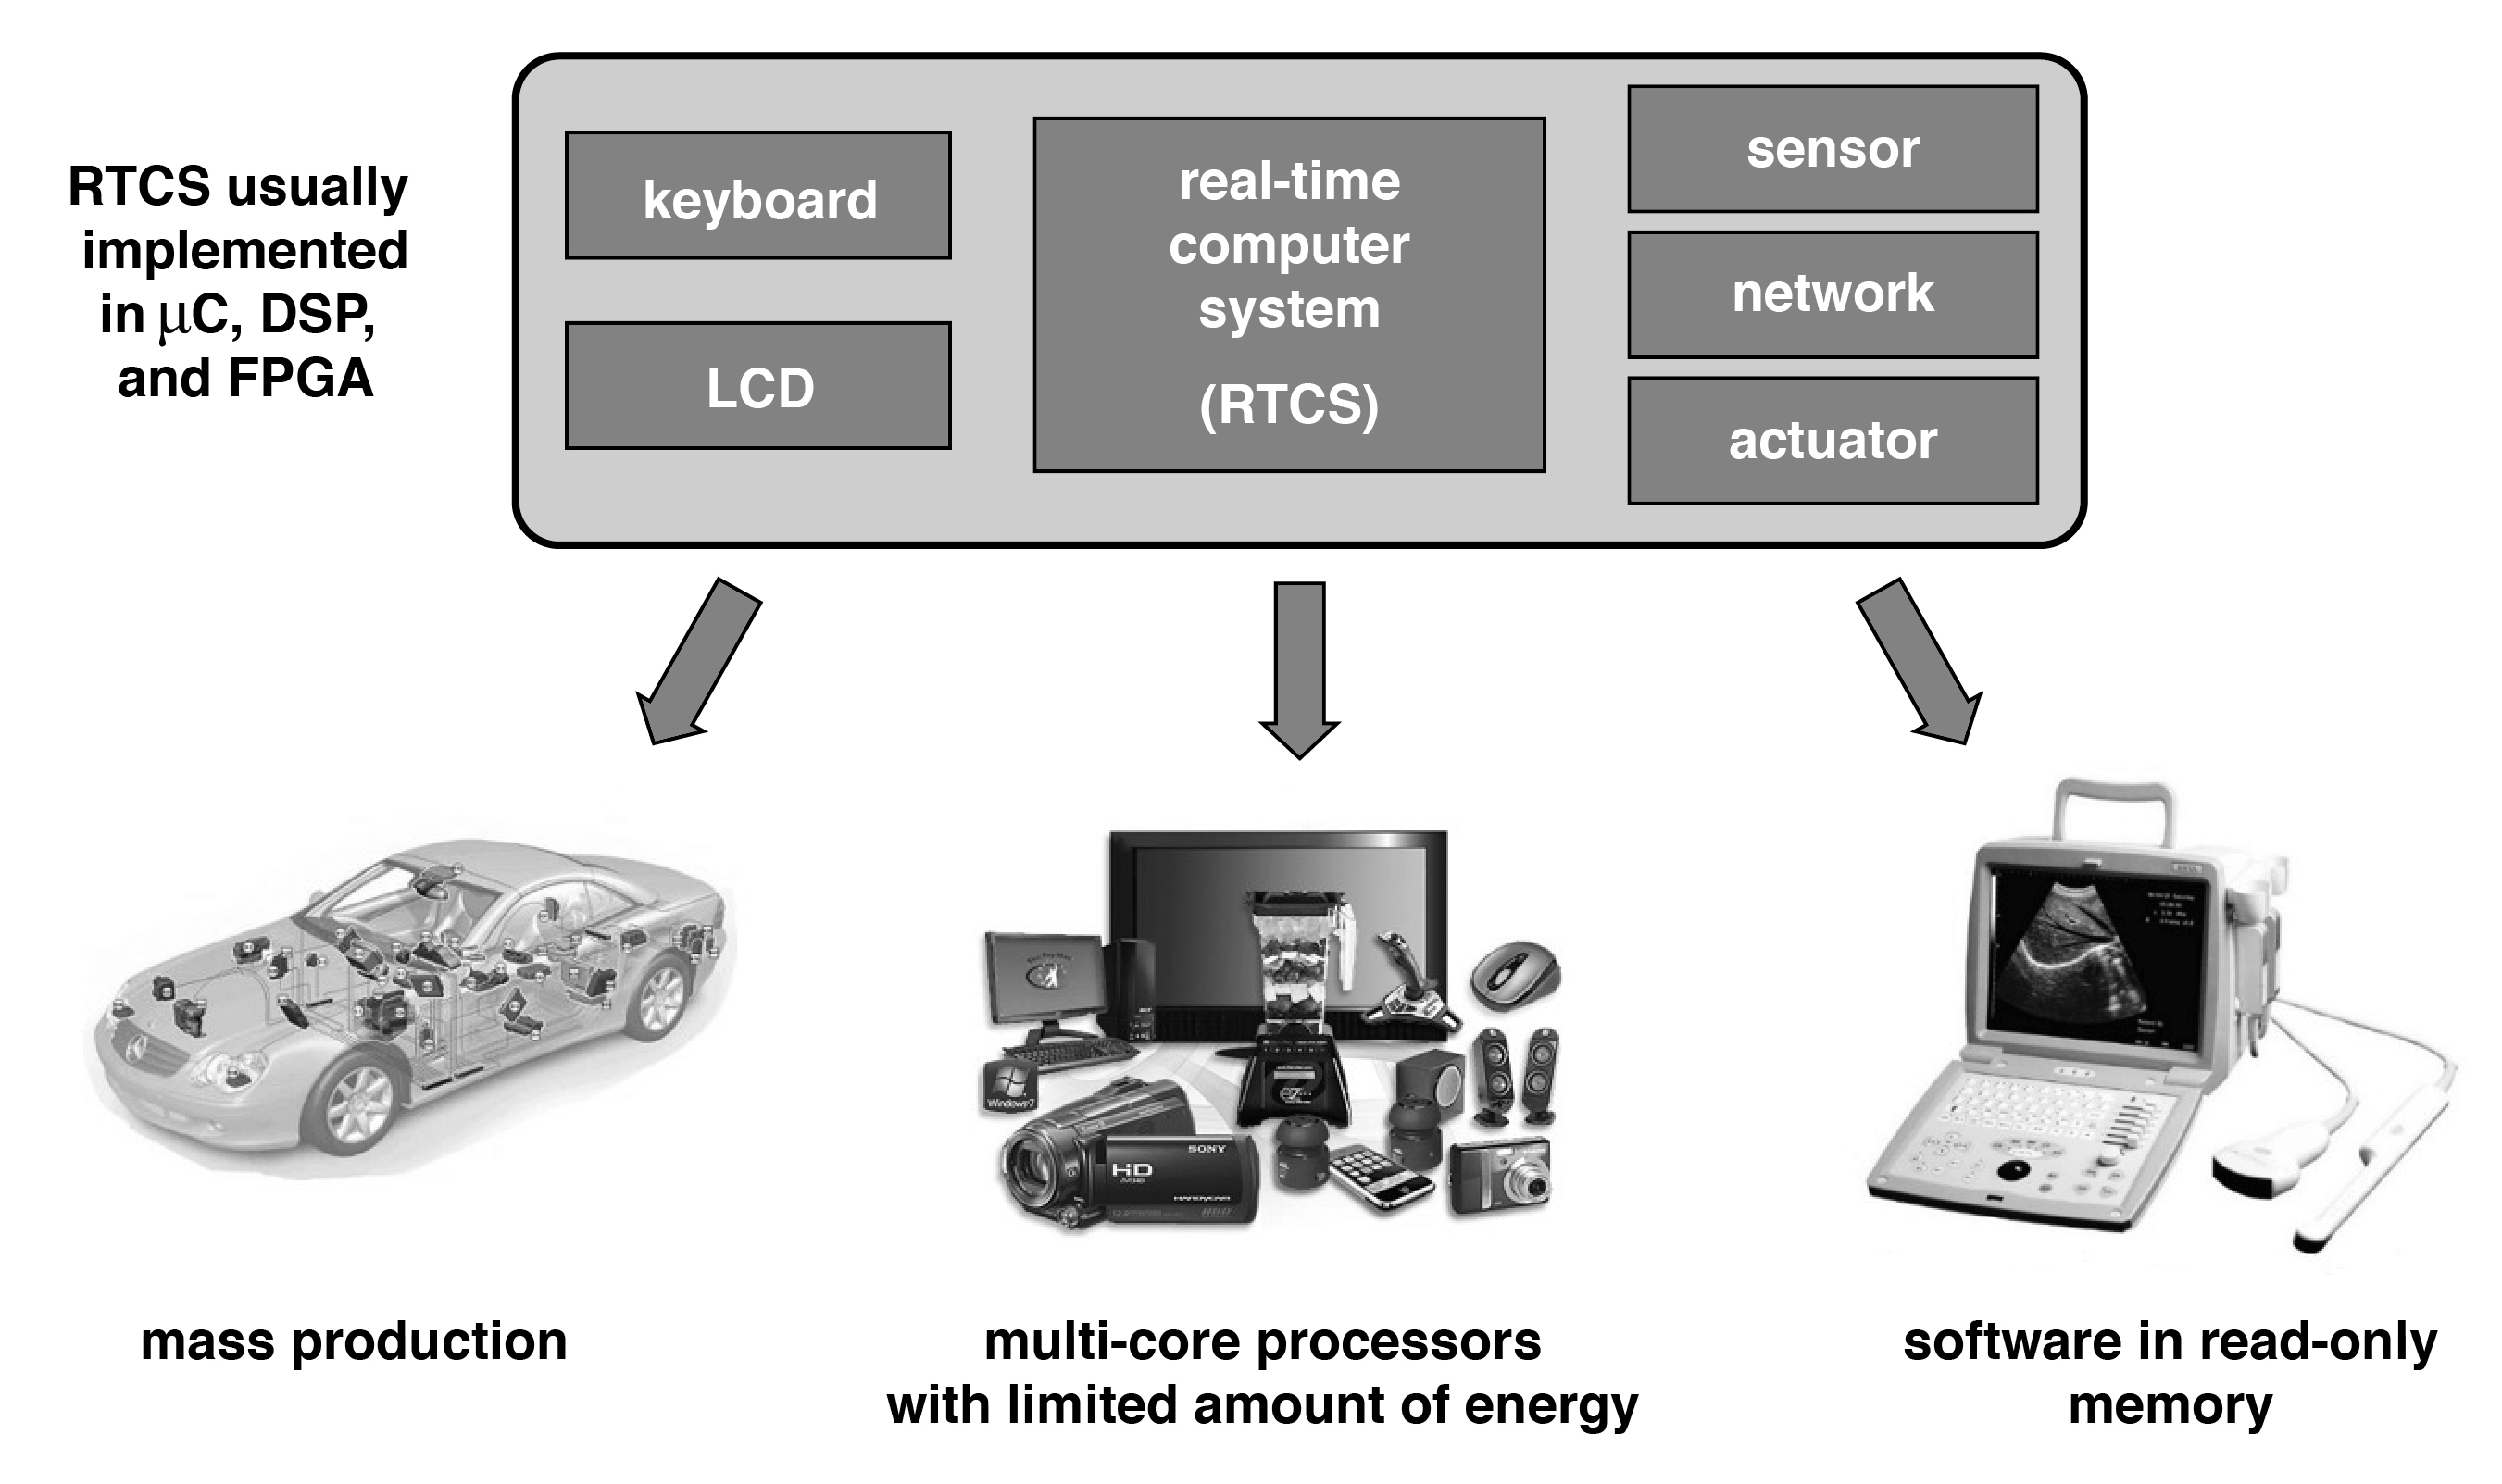
\includegraphics[scale=0.35]{figure1.eps}
	\caption{An embedded system is part of a well-specified larger system (intelligent product).}
	\label{intelligent-product}
\end{figure}

Besides, when physical interaction with the real world is needed, which happens in CPSs, additional care must be taken, mainly when human action is directly replaced, as in vehicle driving. Regarding the latter, even human-in-the-loop feedback control can be employed \cite{munir}, which then raises deeper concerns related to the reliability of human behavior modeling and system implementation. Consequently, it is important to go beyond design correctness and also address behavior correctness, which may be performed by incorporating system models. Specifically, such models can be used to synthesize a given particular system, by ensuring that all needed functions are correctly implemented and the correct behavior is exhibited, {i.e.}, the system is indeed correct by its method of construction~\cite{Abate17}.

For instance, one may argue that a Linux device driver \cite{ldd} was verified and correctly uses the related kernel services; however, not much can be said about correct access to the associated hardware and its use, {\it i.e.}, if read and write operations are performed according to what is specified in the device's datasheet and setup periods are respected. In summary, the main goal would be to ensure that the developed driver is compliant with the underlying hardware, which goes further than code correctness and also tackles the interaction with surrounding entities.

A number of distinctive characteristics might influence the embedded system development and verification process, which include: mass production and static structure, functionality determined by software in read-only memory, multi-core processors with scalable shared memory, and limited amount of energy. Additionally, the increasing computational power and decreasing size and cost, which are common to the area of computer processors, are enabling system designers to move more features to software domain, which consequently leads to difficulties in verifying design correctness, since stringent constraints imposed by the underlying hardware ({\it e.g.}, real-time, memory allocation, interrupts, interfacing, and concurrency) must be considered during verification~\cite{Kroening15}. Such observations expand the addressed issues and even complement what was mentioned in the last paragraphs.

The goals of the present article is to briefly present part of the established research and also clarify the current trends, which are mainly driven by CPSs and IoT. We present a brief discussion about models for CPS, in Section \ref{sec:model}, and then cover preliminaries on bounded model checking, \textit{k}-induction verification based on invariant inference, and counter-example guided inductive synthesis, in Section~\ref{Preliminaries}. In Section~\ref{Verification-Challenges}, the main challenges regarding the verification and synthesis of embedded systems are described, while Section~\ref{Research-Problem} tackles those challenges that are (partially) open in current published research. Section \ref{Newapp} then addresses new applications, which take into account the new trends mentioned here, and Section~\ref{achievements} describes current achievements and future trends in verification and synthesis of embedded systems. Finally, we conclude and describe future work in Section~\ref{conclusions}.

%--------------------------------------
\section{A model for Cyber-physical systems}
\label{sec:model}
%--------------------------------------

Models are largely employed in the science and engineering areas, in order to analyze, predict and modify the behavior of real-world systems. Specially, deterministic and stochastic models are the basis of many engineering advances, in the last centuries. The former is uniquely determined by parameter values and previous states, while the latter presents inherent randomness, which is described by probability distributions. Nonetheless, one can argue that such models are not enough to represent CPSs, because the interaction among software, communications, and hardware presents a lot of events that could not be deterministically or stochastically modeled and may be better represented by nondeterministic approaches~\cite{leeCPS2}. Indeed, that is even more evident when unknown properties are addressed, such as human behavior.

On the one hand, the early representation of hybrid systems, {\it i.e.}, systems that mix continuous and discrete dynamics, consisted in representing discrete components and discretized continuous dynamics by using discrete models and considering non-modeled effects as uncertainties or perturbations exogenous to them, which may even be negligible. On the other hand, that approach is not suitable for complex CPSs that present a lot of nondeterminism, given that uncertainties play a central role.

CPSs have been modeled through different structures that present different degrees of nondeterminism and balance between continuous and discrete dynamics, such as timed automata (\textcolor{red}{CITAR}) and hybrid automata (\textcolor{red}{CITAR}). Rungger and Tabuada (\textcolor{red}{CITAR TAC 2016}) proposed a general and wide model for CPS. Following this proposal, a CPS $S$ is a tuple $S=(X,X_{0},U,r)$, where $X$ is a set of reachable states, $X_{0}$ is a set of initial states, $U$ is a set of inputs, and $r$ is a transition function, such that $r:X\times U \rightarrow X$.

\textcolor{red}{seria legal falar que nondeterminism pode ser tratado com model checking}

%--------------------------------------
\section{Bounded Model Checking (BMC)}
\label{Preliminaries}
%--------------------------------------

Bounded Model Checking (BMC) based on Boolean Satisfiability (SAT) was originally proposed to verify hardware designs~\cite{Biere99,handbook09}. Indeed, Biere {\it et al.} were able to successfully verify large digital circuits with approximately $9510$ latches and $9499$ inputs, leading to BMC formulae with $4 \times 10^6$ variables and $1.2 \times 10^7$ clauses to be checked by standard SAT solvers. BMC based on Satisfiability Modulo Theories (SMT)~\cite{BarrettSST09}, in turn, was originally proposed to deal with increasing software verification complexity~\cite{Armando06}. 

In general, BMC techniques aim to check the violation of a given (safety) property at a given system depth, as shown in Figure~\ref{bounded-model-checking}. Indeed, given a transition system \textit{M}, which is derived from the control-flow graph of a program, a property $\phi$, which represents program correctness and/or a system's behavior, and an iteration bound \textit{k}, which limits loop unrolling, data structures, and context-switches, BMC techniques thus unfold a system \textit{k} times, in order to convert it into a verification condition $\psi$, which is expressed in propositional logic or in a decidable-fragment of first-order logic, such that $\psi$ is \textit{satisfiable} if and only if $\phi$ has a counterexample of depth less than or equal to \textit{k}.

\begin{figure}[h]
	\centering
	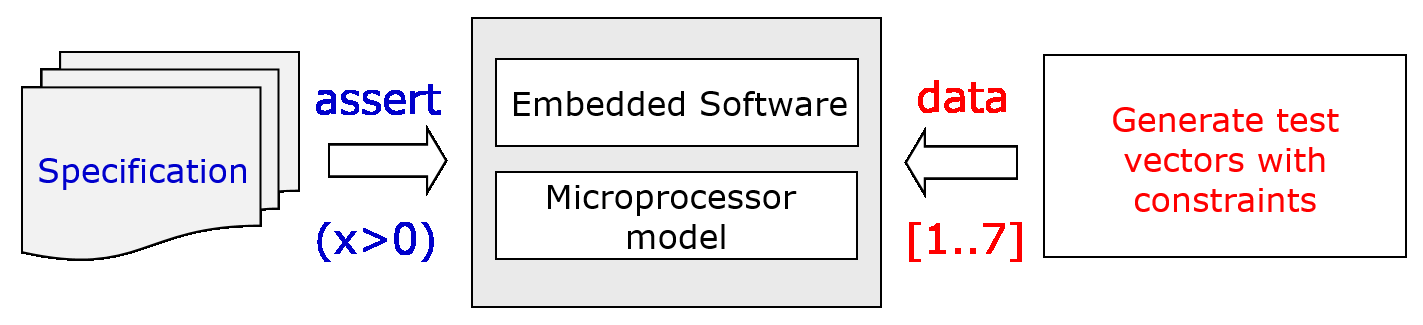
\includegraphics[scale=0.35]{figure2.eps}
	\caption{Bounded Model Checking.}
	\label{bounded-model-checking}
\end{figure}


From the practical point of view, SAT-based or SMT-based BMC procedures have been successfully applied to verify a large number of hardware and software systems, including digital circuits and single- and multi-threaded programs. Those BMC techniques were able to find subtle bugs in real digital and embedded software systems, as reported in the available literature~\cite{Clarke04,MerzFS12,CordeiroF11,Ivancic05,Cordeiro12}. Nonetheless, the main criticism with respect to BMC techniques relies on completeness, since they are able to prove system correctness only if an upper bound \textit{k} is known, {\it i.e.}, a bound that unfolds all loops and recursive functions to their maximum possible depth. 

Due to that limitation, BMC tools are typically susceptible to exhaustion of time or memory limits, when checking complex circuit-implementations or programs with loops, whose bounds are too large or cannot be statically determined.  

%--------------------------------------
\subsection{Induction-based Verification of C Programs}
%--------------------------------------

One promising approach to achieve completeness, in BMC techniques, is to prove that an invariant (assertion) is \textit{k}-inductive~\cite{EenS03,Sheera00}. The main challenge, however, of such an approach relies on computing and strengthening inductive invariants from programs. In particular, loop invariants, which are computed from programs under verification, must be inductive (and not just invariant), in order to validate the corresponding verification conditions, {\it i.e.}, induction cannot determine the invariance of a non-inductive assertion~\cite{Bradley07}. As a consequence, even if \textit{k}-induction procedures successfully compute such assertions, which are indeed invariant, those must be inductive, so that verifiers can automatically prove program correctness.

There are several invariant-generation algorithms that discover linear and polynomial relations among integer and real variables, in order to provide loop invariants and also discover the memory ``shape'', in programming languages with pointers~\cite{pips:2013,Henry:2012}. The current literature also reports successful applications of \textit{k}-induction based verification algorithms for hardware and software systems, using invariant generation and strengthening, mostly based on interval analysis. \textcolor{red}{eh bom citar essa literatura aqui} 

Novel verification algorithms for proving correctness of (a large set of) C programs, by mathematical induction and in a completely automatic way ({\it i.e.}, users do not need to provide loop invariants), were recently proposed~\cite{Gadelha15,Beyer15,Brain15,Rocha15,Kinductor,Rocha17}. Additionally, \textit{k}-induction based verification was also applied to ensure that (restricted) C programs (1) do not contain violations related to data races~\cite{Donaldson10}, considering the Cell BE processor, and (2) do respect time constraints, which are specified during system design phases~\cite{EenS03}. Apart from that, \textit{k}-induction is also a well-established technique in hardware verification, where it is easily applied, due to the monolithic transition relation present in such designs~\cite{EenS03,Sheera00,GrosseLD09}.

It is worth noticing that \textit{k}-induction with invariants has the potential to be directly integrated into existing BMC approaches, given that the induction algorithm itself can be seen as an extension after \textit{k} unwindings and it is possible to generate program invariants with other software modules, which are then translated and instrumented into an input program \cite{Rocha15}.

Nonetheless, there is~little evidence, in the available literature, that model checking hardware and software systems through \textit{k}-induction (and invariants) can be efficiently exploited in embedded-system verification. That happens due to the distinctive characteristics mentioned earlier, which influence the embedded system development and also the employed verification processes. Additionally, there is still a lack of studies for embedded software verifiers to exploit the combination of different invariant generation and strengthening algorithms, including analysis to discover linear inequalities, polynomial equalities and inequalities, and invariants related to memory and variable aliasing~\cite{Bradley07}.

%--------------------------------------
\subsection{Program Synthesis via Counter-Example \\ Guided Inductive Synthesis (CEGIS)}
%--------------------------------------

The basic idea of program synthesis is to automatically construct a program $P$ that satisfies a correctness specification $\sigma$. In particular, program synthesis is automatically performed by engines that use a correctness specification $\sigma$ as the starting point, and then incrementally produce a sequence of candidate solutions that satisfy $\sigma$~\cite{Abate17}. As a result, a given candidate program $p$ is iteratively refined, in order to match the specification $\sigma$ more closely. Counter-Example Guided Inductive Synthesis (CEGIS) represents one of the most popular approaches to program synthesis that are currently used in practice~\cite{David15}. Figure~\ref{Counter-Example-Guided-Inductive-Synthesis} shows the basic architecture of the CEGIS approach, which has close connections to algorithmic debugging using counterexamples and abstraction refinement~\cite{Alur13}. 

The correctness specification $\sigma$ provided to the program synthesizer is of the form $\exists \vec{F} .  \forall \vec{x}.  \sigma(\vec{x}, \vec{F})$, where $\vec{F}$ ranges over functions, $\vec{x}$ ranges over ground terms, and $\sigma$ is a quantifier-free formula typically supported by SMT solvers. The ground terms are interpreted over some finite domain $\mathcal{D}$, where $\mathcal{D}$ can be encoded using the SMT's bit-vectors part. The {\sc Synthesize} and {\sc Verify} phases interact via a finite set of test vectors {\sc inputs} that is updated incrementally. Given the correctness specification $\sigma$, the {\sc Synthesize} procedure tries to find an existential witness $\vec{F}$ satisfying the specification $\sigma(\vec{x}, \vec{F})$, for all $\vec{x}$ in {\sc inputs} (as opposed to all $\vec{x} \in \mathcal{D}$). If {\sc synthesize} succeeds in finding a witness~$\vec{F}$, this witness is a candidate solution to the full synthesis formula, which is passed to the {\sc verify} phase, in order to check whether it is a full solution ({\it i.e.}, $\vec{F}$ satisfies the specification $\sigma(\vec{x}, \vec{F})$ for all $\vec{x}\in\mathcal{D}$). If this is the case, then the algorithm terminates; otherwise, additional information is provided to the {\sc synthesize} phase, in the form of a new counterexample that is added to the {\sc inputs} set and the loop iterates again. 
%
\begin{figure}[h]
	\centering
	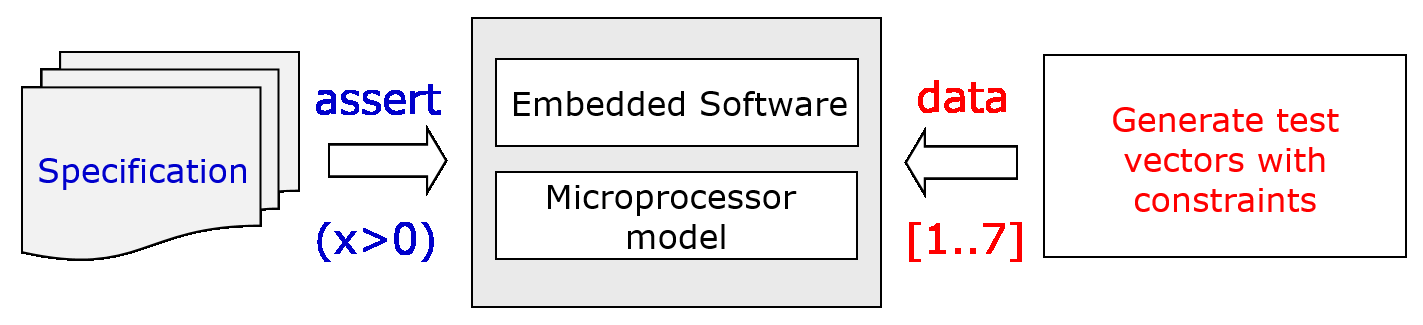
\includegraphics[scale=0.12]{figure4.eps}
	\caption{Counter-Example Guided Inductive Synthesis.}
	\label{Counter-Example-Guided-Inductive-Synthesis}
\end{figure}

Note that each iteration of the CEGIS loop adds a new input to the finite set $\text{\sc inputs}$ that is used for synthesis.  Given that the full set of inputs $\mathcal{D}$ is finite, this means that the refinement loop can only iterate a finite number of times; however, $\mathcal{D}$ can represent a large number of elements for the finite set $\text{\sc inputs}$. In order to avoid exploring all possible values, machine learning techniques can be used in the {\sc Synthesize} phase, with the goal of learning from experience, {\it i.e.}, learning from counterexamples provided by a verification oracle~\cite{Alur13}.

Nowadays, program synthesis engines that implement CEGIS approach~\cite{sketch} can automatically produce solutions for a large variety of specifications, due to the combination of automated testing, genetic algorithms, and SMT-based automated reasoning~\cite{Sharma14}.

%--------------------------------------
\subsection{Incorporating System Models to Automated \\ Verification and Synthesis Procedures}
%--------------------------------------

Currently, SMT-based BMC approaches check code properties in real programs, which basically address programing-language issues and general correctness, without taking into account target applications or system behavior. Such a statement is important, since, as already mentioned, many system features are being moved to software domain, which then requires schemes that do not only check if source code is correctly written, but also if it will properly respond in real environments or under external problems. For instance, the anti-lock braking system software of a vehicle model can be bug free, but it may not work correctly if a sensor is damaged.

Indeed, research in software verification is now incorporating such considerations, during checking processes, and some schemes already use knowledge about the system to be verified and the underlying hardware. Recently, a verification tool for digital systems was proposed, which is called digital system verifier (DSVerifier)~\cite{dsv_spin2015,Monteiro16} and is able to aid engineers to check overflow, limit cycle, output error, timing, stability, and minimum phase, considering finite word-length (FWL) effects. Additionally, DSVerifier checks closed-loop systems with uncertain models considering FWL effects, which are typically represented as hybrid systems, {\it i.e.}, the controller is digital but the controlled agent (plant) is a physical and continuous system~\cite{Bessa17}. That ultimately leads to the use of analog-to-digital converters, which are one of the most important aspects to be considered, given that data loss (quantization) is inevitable. As a consequence, the verification procedure has to consider the interaction between a continuous plant and a digital (and sampled) controller with FWL effects, which can be connected using different control system configurations. Additionally, the latter may present a different behavior, regarding what was specified in analog domain, due to the inherent discret-time operation. 


In summary, DSVerifier is a useful test tool, which takes into account different representations ({\it e.g.}, transfer-function and state-space), realization forms ({\it e.g.}, direct forms, delta forms, and transposed forms) and other implementation restrictions, in order to explore the design space. Finally, if a system's requirements are not met with a given configuration, an analysis of the provided error report may suggest another setup. 

In this respect, DSVerifier has been extended to automatically synthesize digital stabilizing controllers for continuous plants~\cite{Abate17}. In particular, a CEGIS-based approach, implemented in a tool called digital system synthesizer (DSSynth), uses inductive synthesis in conjunction with DSVerifier's algorithm for verifying robust closed-loop stability that addresses plant variations as interval sets, as well as FWL uncertainties in digital controllers. DSSynth is able to successfully synthesize stable digital controllers for a set of intricate plant models, taken from the control literature, within minutes.

Apart from the control system domain, Scratch is another example software model-checking tool, which uses knowledge about the system to be verified and the underlying hardware, with the goal of detecting races related to direct memory access (DMA), in the Cell BE processor~\cite{Donaldson10}. That tool also uses BMC, in order to detect DMA races, and BMC with \textit{k}-induction, which aims to prove the absence of races. If support to other DMA operations were added, Scratch could be adapted to different architectures, {\it i.e.}, the same techniques would be employed, but with a different system behavior/knowledge.

One may also notice that such a paradigm, {\it i.e.}, verification and synthesis based on an expected system behavior, is not restricted to digital filters and controllers or DMA races, but it can also by applied to possibly any real system, as long as the desired behavior can be expressed as properties in BMC frameworks. For instance, regarding self-driving cars, a property could be the detection of pedestrians or animals, or even bicycles. Indeed, the latter is considered one of the most difficult problems, due to the myriad of possible shape and colors \cite{selfcar}. In addition, the mentioned problem is closely related to machine learning, from which refinement strategies can be devised \cite{BMCml}. 


%--------------------------------------
\section{Verification and Synthesis \\ Challenges for Embedded Systems}
\label{Verification-Challenges} 
%--------------------------------------

Generally, state-of-the-art verification methodologies for embedded systems generate test vectors (with constraints) and use assertion-based verification and high-level processor models, during simulation~\cite{Behrend15,Lettnin09}, as shown in Figure~\ref{verification-methodologies}. 
%
\begin{figure}[h]
	\centering
	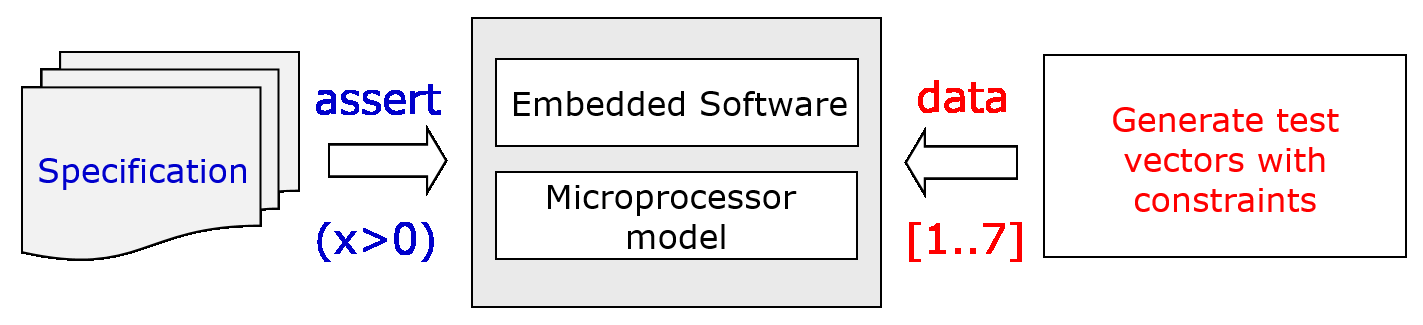
\includegraphics[scale=0.35]{figure3.eps}
	\caption{Verification methodologies for embedded systems.}
	\label{verification-methodologies}
\end{figure}


In particular, the main challenges regarding verification of embedded systems lie on improving coverage, where more system functions are verified, reducing verification time, {\it i.e.}, pruning the state-space exploration during verification, providing completeness, {\it i.e.},  if all possible states can be reached and evaluated, and incorporating system models, which allow specific checks regarding system behavior and not only code correctness. Additionally, embedded system verification raises additional challenges, such as 
%
\begin{enumerate}
	\item time and energy constraints.
	\item handling of concurrent software.
	\item platform restrictions.
	\item verification of code pieces or modules that rely on larger structures.
	\item legacy designs. %, which are usually developed with low-level languages.
	\item support to different programming languages, frameworks, and interfaces.
	\item correct code instrumentation.
	\item handling of non-linear and non-convex optimization problems.
\end{enumerate}

Indeed, the first two aspects are of extreme relevance in micro-grids and cyber-physical systems, in order to ensure reliability, which is a key issue for (smart) cities, industries, and consumers, and the third one is essential in systems that implement device models, such as digital filters and controllers, which present a behavior that is highly dependent on signal inputs and outputs and whose deployment may be heavily affected by hardware restrictions. The fourth aspect deals with code that relies on existing infrastructures and must be compliant with those, such as Linux kernel modules. The fifth aspect, in turn, is inherent to a large number of embedded systems from  telecommunications, control systems, and medical devices. In particular, software developed for that type of embedded systems has been extensively tested and verified, and also optimized for efficiency over years of development. Therefore, when a new product is derived from a given platform, a lot of legacy code is usually reused for improving development time and code quality. The sixth aspect is related to the evolution of development processes and technologies, which may delay the application of suitable verification and synthesis approaches, if verifiers and synthesizers do not support different programming languages and interfaces. The seventh aspect highlights a subjective task in verification: where one must insert an evaluation point or assertion, in order to correct address a property. Finally, the last one is related to the widespread use of embedded systems in autonomous-vehicle navigation systems~\cite{Adouane16}, which demands optimization solving during their execution for a wide range of functions, including non-linear and non-convex problems using fixed- and floating-point arithmetic.

Those eight challenges place additional difficulties for developing reliable synthesizers for embedded systems, especially for cyber-physical systems and micro-grids, where the controlled object ({\it e.g.}, physical plant) typically exhibits continuous behavior, whereas the controller (usually implemented by a real-time computer system) operates in discrete time and over a quantized domain. In particular, synthesizers for those systems need to consider the effects of quantizers (A/D and D/A converters), when a digital equivalent of the controlled object is considered, {\it i.e.}, a model of their physical environment (cf. intelligent product in Figure~\ref{intelligent-product}). Additionally,  finite-precision arithmetic and their related rounding errors need to be considered, when correct-by-construction code is generated for embedded systems.

%--------------------------------------
\section{Research Problem (RP)}
\label{Research-Problem}
%--------------------------------------

This position paper tackles seven major problems in computer-aided verification and synthesis for embedded systems, which are (partially) open in current published research.

\textbf{(RP1)} provision of suitable encoding into SMT \cite{BarrettSST09}, which may extend the background theories typically supported by SMT solvers, with the goal of reasoning accurately and effectively about realistic embedded programs.

\textbf{(RP2)} exploitation of SMT techniques to leverage bounded model checking of multi-threaded software, in order to mitigate the state-explosion problem due to thread interleaving.
	
\textbf{(RP3)} proof of correctness and timeliness of embedded systems, by taking into account stringent constraints imposed by hardware.
	
\textbf{(RP4)} incorporation of knowledge about system purpose and associated features, which aims to detect system-level and behavior failures.

\textbf{(RP5)} provision of tools and approaches capable of addressing different programming languages and application interfaces, with the goal of reducing the time needed to adapt current verification techniques to new developments and technologies.

\textbf{(RP6)} development of automated synthesis approaches that are algorithmically and numerically sound, in order to handle (control) software that is tightly coupled with the physical environment by considering uncertain models and FWL effects.

\textbf{(RP7)} provision of a unified framework, which is able to tackle high and low level properties, as well as system behavior, with the potential to lead to another degree of completeness, in such a way that every implementation aspect of an embedded system is addressed and evaluated.


Section~\ref{achievements} outlines contributions toward these research problems.



%--------------------------------------
\section{Current Achievements and \\ Future Trends}
\label{achievements}
%--------------------------------------

\textbf{(RP1)} Cordeiro, Fischer, and Marques-Silva proposed the first SMT-based BMC for full C programs, called Efficient SMT-Based Context-Bounded Model Checker (ESBMC)~\cite{Cordeiro12}, which was later extended to support C++98 programs~\cite{ECBS13}, CUDA programs~\cite{Pereira15}, and Qt-based consumer electronics applications~\cite{Sousa15}. This approach was also able to find undiscovered bugs related to arithmetic overflow, buffer overflow, and invalid pointer, in standard benchmarks, which were later confirmed by the benchmarks' creators ({\it e.g.}, NOKIA, NEC, NXP, and VERISEC)~\cite{CordeiroF11,Cordeiro12}. Other SMT-based BMC approaches have also been proposed and implemented~\cite{MerzFS12}, but the coverage and verification time of all existing ones are still limited to specific classes of programs, especially for those that contain intensive floating-point arithmetic and dynamic memory allocation~\cite{Beyer14,BeyerSVCOMP15}. One possible research direction is to bridge the gap between BMC tools and SMT solvers to propose background theories and develop more efficient decision procedures, in order to handle specific classes of programs.

\textbf{(RP2)} The SMT-based BMC approach proposed by Cordeiro, Fischer, and Marques-Silva was further developed to verify correct lock acquisition ordering and the absence of deadlocks, data races, and atomicity violations in multi-threaded software based on POSIX and CUDA libraries~\cite{CordeiroF11,Pereira15}, considering monotonic partial-order reduction~\cite{KahlonWG09} and state-hashing techniques, in order to prune the state-space exploration~\cite{morse15}. Recent advances for verifying multi-threaded C programs have been proposed to speed up the verification time, which significantly prune the state-space exploration~\cite{Inverso14,civl15}; however, the class of concurrent programs ({\it e.g.}, CUDA, OpenCL, and MPI) that can be verified is still very limited. One possible research direction is to further extend BMC of multi-threaded C programs via Lazy Sequentialization~\cite{Inverso14}, in order to analyze unsatisfiability cores~\cite{Grumberg05} with the goal to remove redundant behaviour or to analyze interpolants~\cite{McMillan11} to prove non-interference of context switches.

\textbf{(RP3)} Novel approaches to model check embedded software using \textit{k}-induction and invariants were proposed and evaluated in the literature, which demonstrate its effectiveness in some real-life embedded-system applications~\cite{Gadelha15,Brain15,Rocha15,Donaldson10,Rocha17}; however, the main challenge still remains open, {\it i.e.}, to compute and strengthen loop invariants to prove program correctness and timeliness in a more efficient and effective way, in order to be competitive with other model-checking approaches. In particular, invariant-generation algorithms have substantially evolved over the last years, with the goal of discovering inductive invariants of programs~\cite{pips:2013,Henry:2012} or continuously refine them during verification~\cite{Beyer15}; however, there is still a lack of studies for exploiting the combination of different invariant-generation algorithms ({\it e.g.}, interval analysis, linear inequalities, polynomial equalities and inequalities) and how to strengthen them during verification, in order to ensure system robustness w.r.t. implementation aspects.

\textbf{(RP4)} State-of-the-art SMT-based context-BMC approaches were extended to verify overflow, limit cycle, time constraints, stability, and minimum phase, in digital systems. Indeed, digital filters and controllers~\cite{dsv_spin2015,esbmc_controller,esbmc_filter} were tackled, in order to specify system-level properties of those systems, using linear-time temporal logic~\cite{JMorse15}. In particular, a specific UAV application was tackled, with the goal to verify its attitude controllers~\cite{Bessa16,Chaves17}. In general, however, there is still a lack of studies to verify system-level properties related to embedded systems; emphasis should be given to micro-grids~\cite{xu15} and cyber-physical systems~\cite{leeCPS2}, which require high-dependability requirements for computation, control, and communication. Additionally, the application of automated fault detection, localization, and correction techniques to digital systems represents an important research direction to make BMC tools useful for embedded systems engineers~\cite{Alves15}.

{\textbf{(RP5)} Although ESBMC \cite{Cordeiro12} was extended to support C/C++ and some variants, new application interfaces and programming languages are often developed, which require suitable software verification tools. Indeed, it would be interesting if a new programming language model could be loaded, which along with a BMC core could check different programs. Some work towards that was already presented by Sousa, Cordeiro, and Filho~\cite{Garcia16}, which employed operational models for checking Qt-based programs from consumer electronics. In summary, the BMC core (in that case, ESBMC) is not changed, but instead an operational model, which implements the behavior and features of Qt libraries, is used for providing the new code structure to be checked. Such research problem is closely related to the first one \textbf{(RP1)} and has the potential to devise a new paradigm in software verification.

{\textbf{(RP6)} State-of-the-art synthesis approaches for embedded (control) systems typically disregard the platform in which the embedded system software operates and restrict itself to generate code that do not take into account FWL effects. The synthesized system, however, must include the physical plant to avoid serious system's malfunctioning (or even a catastrophe) due to the embedded (control) software, {\it e.g.}, the Mars Polar Lander did not account for leg compressions prior to landing~\cite{Jackson16}. Research in this direction has made some progress to design, implement, and evaluate an automated approach for generating correct-by-construction digital controllers that is based on state-of-the-art inductive synthesis techniques~\cite{Abate17}. However, there is still little evidence whether that approach can scale for larger systems modeled by other types of representations ({\it e.g.}, state-space). In addition to that, another research direction for synthesizers is to generate code for UAV trajectory and mission planning by taking into account system's dynamics and nonholonomic constraints~\cite{Araujo16}. As a consequence, verifiers and synthesizers need to handle a wide range of functions, including non-linear and non-convex optimization problems based on both fixed- and floating-point arithmetic.

Lastly, yet importantly, BMC tools like CBMC~\cite{Clarke04}, ESBMC~\cite{MorseCNF13,MorseRCN014}, SMACK~\cite{Haran15}, and LLBMC~\cite{MerzFS12} represent the most prominent approaches for verifying C programs, as observed in the Intl. Competition on Software Verification~\cite{Beyer14,BeyerSVCOMP15,Beyer16}, where verifiable (correctness and violation) witnesses are of extreme importance for evaluating software verifiers~\cite{BeyerW15,RochaIFM12}. The increasing number of verification tasks being added every year to the competition allows developers to further improve their verifiers by implementing new types of abstraction and simplification techniques. As a consequence, the continuous development and improvement of verifiers can leverage more efficient synthesizers and increase further the reliability of the verified (embedded) system.

\section{New Applications: Beyond Code Correctness}
\label{Newapp}


%--------------------------------------
\section{Conclusions}
\label{conclusions}
%--------------------------------------

This paper presented the main challenges related to the verification of design correctness, in embedded systems, and also raised some important side considerations about synthesis. In particular, it emphasizes that stringent constraints imposed by the underlying hardware ({\it e.g.}, real-time, memory allocation, interrupts, and concurrency), along with system behavior models, must be considered during verification and synthesis. Additionally, there is little evidence that model checking embedded software using \textit{k}-induction (and invariants), which
extends BMC-based approaches from falsification to verification, can be applied to formally verify correctness and timeliness of embedded systems. 

Given that software complexity has significantly increased in embedded products, there are still some (recent) advances to stress and exhaustively cover the system state space, in order to verify low-level properties that have to meet the application's deadline, access memory regions, handle concurrency, and control hardware registers. Besides, there is a trend towards incorporating knowledge about the system to be verified, which may take software verification and synthesis one step further, where not only code correctness will be addressed, but also full system reliability. Finally, it seems interesting to provide behavioral models when new application interfaces or programming language features are used, in order to extend the capabilities of current verification tools, without changing the core BMC module.

As future work, the main goal of this research is to extend BMC as a design, verification, and synthesis tool for achieving correct-by-construction embedded system implementations. Special attention will be given to cyber-physical systems and modern micro-grids, considering small-scale versions of a distributed system, so that reliability and other system-level properties ({\it e.g.}, carbon emission reduction in smart cities) are amenable to automated verification, probably through behavior models.



% conference papers do not normally have an appendix


% use section* for acknowledgment
%\section*{Acknowledgment}

%The authors would like to thank...
%The authors thank M. Dangl for reviewing a draft version of this paper.~This research was supported by CNPq $475647$/$2013$-$0$ grant.



\begin{thebibliography}{1}

%1
\bibitem{Kopetz11}
H.~Kopetz:
\newblock {\em {Real-Time Systems - Design Principles for Distributed Embedded Applications}}.
\newblock Real-Time Systems Series, Springer, ISBN 978-1-4419-8236-0, pp. 1--376, 2011.

%2
\bibitem{xu15}
Xua X., Jiaa H., Wanga D., Yub D., Chiangc H.:
\newblock {\em {Hierarchical energy management system for multi-source multi-product microgrids}}.
\newblock In: Renewable Energy, v. 78, pp. 621--630, 2015.

%3
\bibitem{leeCPS}
Lee E.:
\newblock {\em {Cyber-physical Systems: Design Challenges}}.
\newblock In: International Symposium on Object Oriented Real-Time Distributed Computing, pp. 363--369, 2008.

%4
\bibitem{leeCPS2}
Lee E.:
\newblock {\em {The Past, Present and Future of Cyber-Physical Systems: A Focus on Models}}. 
\newblock In: Sensors 15(3): pp. 4837--4869, 2015.

%5
\bibitem{groza2015formal}
Groza A., Letia I., Goron A., Zaporojan S.: 
\newblock {\em {A formal approach for identifying assurance deficits in unmanned aerial vehicle software}}.
\newblock In: Progress in Systems Engineering, Springer, pp. 233--239, 2015.

%6
\bibitem{Cordeiro09}
Cordeiro L., Fischer B., Chen H., Marques-Silva J.:
\newblock {\em {Semiformal Verification of Embedded Software in Medical Devices Considering Stringent Hardware Constraints}}.
\newblock In: International Conference on Embedded Software and Systems, pp. 396--403, 2009.

%7
\bibitem{munir}
Munir S., Stankovic J. A., Liang C.-J. M., Lin S.:
\newblock {\em {Cyber Physical System Challenges for Human-in-the-Loop Control}}. 
\newblock In: 8th International Workshop on Feedback Computing, pp. 1--4, 2013.

%8
\bibitem{Abate17}
Abate A., Bessa I., Cattaruzza D., Cordeiro L., David C., Kesseli P., Kroening D.:
\newblock {\em {Sound and Automated Synthesis of Digital Stabilizing Controllers for Continuous Plants}}.
\newblock In: 20th ACM International Conference on Hybrid Systems: Computation and Control, 2017 (to appear).

\bibitem{ldd}
Witkowski T., Blanc N., Kroening D., Weissenbacher G.:
\newblock {\em {Model checking concurrent linux device drivers}}.
\newblock In: 22nd IEEE/ACM international conference on Automated software engineering, pp. 501--504, 2007.

%9
\bibitem{Kroening15}
Kroening D., Liang L., Melham T., Schrammel P., Tautschnig M.:
\newblock {\em {Effective Verification of Low-Level Software with Nested Interrupts}}. 
\newblock In: Design, Automation and Test in Europe, pp. 229--234, 2015.

%10
\bibitem{Biere99}
Biere A., Cimatti A., Clarke E., Zhu Y.:
\newblock {\em {Symbolic Model Checking without BDDs}}. 
\newblock In: Tools and Algorithms for Construction and Analysis of Systems, LNCS 1579, pp. 193--207, 1999.

%11
\bibitem{handbook09}
Biere A., Heule M., van Maaren H., Walsh T., eds.:
\newblock {\em {Handbook of Satisfiability}}.
\newblock Volume 185 of Frontiers in Artificial Intelligence and Applications., {IOS} Press, 2009.

%12
\bibitem{BarrettSST09}
Barrett C., Sebastiani R., Seshia S.A., Tinelli C.:
\newblock {\em {Satisfiability Modulo Theories}}. 
\newblock In: Volume 185 of Frontiers in Artificial Intelligence and Applications. IOS Press, pp. 825--885, 2009.

%13
\bibitem{Armando06}
Armando A., Mantovani J., Platania L.:
\newblock {\em {Bounded Model Checking of Software Using SMT Solvers Instead of SAT Solvers}}. 
\newblock In: {SPIN} Workshop on Model Checking Software, LNCS 3925, pp. 146-162, 2006.

%14
\bibitem{Clarke04}
Clarke E., Kroening D., Lerda F.:
\newblock {\em {A Tool for Checking {ANSI-C} Programs}}.
\newblock In: Tools and Algorithms for the Construction and Analysis of Systems. LNCS 2988, Springer Berlin Heidelberg, pp. 168--176, 2004.

%15
\bibitem{MerzFS12}
Merz F., Falke S., Sinz C.:
\newblock {\em {{LLBMC}: Bounded Model Checking of {C} and {C++} Programs using a Compiler {IR}}}.
\newblock In: International Conference on Verified Software: Theories, Tools, Experiments. LNCS 7152, pp. 146--161, 2012.

%16
\bibitem{CordeiroF11}
Cordeiro L., Fischer B.:
\newblock {\em {Verifying Multi-threaded Software using {SMT}-based Context-Bounded Model Checking}}.
\newblock In: International Conference on Software Engineering. pp. 331--340, 2011.

%17
\bibitem{Ivancic05}
Ivanicic F., Shlyakhter I., Gupta A., Ganai, M.K.:
\newblock {\em {Model Checking {C} Programs using {F-Soft}}}.
\newblock In: International Conference on Computer Design: VLSI in Computers and Processors, pp. 297--308, 2005.

%18
\bibitem{Cordeiro12}
Cordeiro L., Fischer B., Marques{-}Silva J.:
\newblock {\em {{SMT}-based Bounded Model Checking for Embedded {ANSI-C} Software}}.
\newblock {IEEE} Trans. Software Eng. 38(4), pp. 957--974, 2012.

%19
\bibitem{EenS03}
E{\'{e}}n, N., S{\"{o}}rensson, N.:
\newblock {\em {Temporal Induction by Incremental {SAT} Solving}}.
\newblock Electronic Notes in Theoretical Computer Science 89(4), pp. 543 -- 560, 2003.

%20
\bibitem{Sheera00}
Sheeran M., Singh S., St{\aa}lmarck G.:
\newblock {\em {Checking Safety Properties using Induction and a {SAT}-solver}}.
\newblock In: International Conference on Formal Methods in Computer-Aided Design. Springer-Verlag, pp. 108--125, 2000.

%21
\bibitem{Bradley07}
Bradley A., Manna Z.:
\newblock {\em {The calculus of computation - decision procedures with applications to verification}}. 
\newblock In: Springer, pp. I-XV, pp. 1--366, 2007.

%22
\bibitem{pips:2013}
ParisTech M.:
\newblock {\em {PIPS: Automatic Parallelizer and Code Transformation Framework}}. 
\newblock Accessed 21 February 2016

%23
\bibitem{Henry:2012}
Henry J., Monniaux D., Moy M.: 
\newblock {\em {PAGAI: A Path Sensitive Static Analyser}}. 
\newblock In: Electronic Notes in Theoretical Computer Science, pp. 15--25, 2012.

%24
\bibitem{Gadelha15}
Gadelha M., Ismail H., Cordeiro L.:
\newblock {\em {Handling Loops in Bounded Model Checking of C Programs via \textit{k}-Induction}}.
\newblock In: International Journal on Software Tools for Technology Transfer (to appear), 2015.
\newblock http://dx.doi.org/10.1007/s10009-015-0407-9

%25
\bibitem{Beyer15}
Beyer D., Dangl M., Wendler P.:
\newblock {\em {Boosting \textit{k}-Induction with Continuously-Refined Invariants}}.
\newblock In: International Conference on Computer-Aided Verification, LNCS 9206, pp. 622--640, 2015.

%26
\bibitem{Brain15}
Brain M., Joshi S., Kroening D., Schrammel P.:
\newblock {\em {Safety Verification and Refutation by k-Invariants and \textit{k}-Induction}}.
\newblock In: International Symposium on Static Analysis, LNCS 9291, pp. 145--161, 2015.

%27
\bibitem{Rocha15}
Rocha H., Ismail H., Cordeiro L., Barreto R.:
\newblock {\em {Model Checking Embedded C Software using \textit{k}-Induction and Invariants}}.
\newblock In: V Brazilian Symposium on Computing Systems Engineering, pp. 90--95, 2015.

%28
\bibitem{Kinductor}
Donaldson A., Haller L., Kroening D., R{\"{u}}mmer, P.:
\newblock {\em {Software Verification using \textit{k}-Induction}}.
\newblock In: International Symposium on Static Analysis. LNCS 6887, pp. 351--368, 2011.

%29
\bibitem{Rocha17}
Rocha, W., Rocha, H., Ismail H., Cordeiro, L., Fischer, B.:
\newblock {\em {DepthK: A \textit{k}-Induction Verifier Based on Invariant Inference for C Programs}}. 
\newblock In: International Conference on Tools and Algorithms for the Construction and Analysis of Systems, 2017 (to appear).

%30
\bibitem{Donaldson10}
Donaldson A., Kroening D., R{\"{u}}mmer P.:
\newblock {\em {{SCRATCH}: A Tool for Automatic Analysis of {DMA} Races}}.
\newblock In: ACM Symposium on Principles and Practice of Parallel Programming. ACM, pp. 311--312, 2011.


\bibitem{selfcar}
Fairley P.:
\newblock {\em {Self-Driving Cars Have a Bicycle Problem}}.
\newblock http://spectrum.ieee.org/transportation/self-driving/selfdriving-cars-have-a-bicycle-problem.


\bibitem{BMCml}
L.~Bortolussi, D. Milios, G, Sanguinetti.:
\newblock {\em {Smoothed model checking for uncertain Continuous-Time Markov Chains}}.
\newblock In:. Information and Computation, 2016.


%31
\bibitem{GrosseLD09}
Gro{\ss}e D., Le H., Drechsler R.:
\newblock {\em {Induction-based Formal Verification of {SystemC TLM} Designs}}.
\newblock In: International Workshop on Microprocessor Test and Verification, pp. 101--106, 2009.

%32
\bibitem{Alur13}
Alur R., Bod\'{\i}k R., Juniwal G., Martin M., Raghothaman M., Seshia S., Singh R., Solar-Lezama A., Torlak E., Udupa A.:
\newblock {\em {Syntax-guided synthesis}}. 
\newblock In: Formal Methods in Computer-Aided Design, pp. 1--8, 2013.

%33
\bibitem{sketch}
A.~Solar-Lezama.
\newblock {\em {Program sketching}}.
\newblock In: International Journal on Software Tools for Technology Transfer, 15(5-6):475--495, 2013.

%34
\bibitem{David15}
C.~David, D.~Kroening, and M.~Lewis.
\newblock {\em {Using program synthesis for program analysis}}.
\newblock In: Logic for Programming, Artificial Intelligence, and Reasoning, LNCS 9450, pp. 483--498, 2015.

%35
\bibitem{Sharma14}
R.~Sharma and A.~Aiken.
\newblock {\em {From invariant checking to invariant inference using randomized search}}.
\newblock In: Computer Aided Verification, LNCS 8559, pp. 88--105, 2014.

%36
\bibitem{dsv_spin2015}
Ismail H., Bessa I., Cordeiro L., Lima Filho E., Chaves Filho J.:
\newblock {\em {DSVerifier: A Bounded Model Checking Tool for Digital Systems}}. 
\newblock In: International SPIN Symposium on Model Checking of Software, LNCS 9232, pp. 126--131, 2015.

%37
\bibitem{Monteiro16}
F.~Monteiro:
\newblock {\em {Bounded model checking of state-space digital systems: the impact of finite word-length effects on the implementation of fixed-point digital controllers based on state-space modeling}}. 
\newblock In: 24th {ACM} {SIGSOFT} International Symposium on Foundations of Software Engineering, pp. 1151--1153, 2016.

%38
\bibitem{Bessa17}
Bessa, I., Ismail, H., Palhares, R., Cordeiro, L., Chaves Filho, J.:
\newblock {\em {Formal Non-Fragile Stability Verification of Digital Control Systems with Uncertainty}}. 
\newblock In: IEEE Transactions on Computers, 2017 (to appear).

%39
\bibitem{Behrend15}
Behrend J., Lettnin D., Gruenhage A., Ruf J., Kropf T., Rosenstiel W.:
\newblock {\em {Scalable and Optimized Hybrid Verification of Embedded Software}}. 
\newblock In: J. Electronic Testing 31(2): pp. 151--166, 2015.

%40
\bibitem{Lettnin09}
Lettnin D., Nalla P. K., Behrend J., Ruf J., Gerlach J., Kropf T., Rosenstiel W., Sch{\"o}nknecht V., Reitemeyer S.:
\newblock {\em {Semiformal Verification of Temporal Properties in Automotive Hardware Dependent Software}}. 
\newblock In: Design, Automation and Test in Europe, pp. 1214--1217, 2009.

%41
\bibitem{Adouane16}
Vilca J., Adouane L., Mezouar Y.:
\newblock {\em {Optimal Multi-Criteria Waypoint Selection for Autonomous Vehicle Navigation in Structured Environment}}. 
\newblock In: Journal of Intelligent and Robotic Systems 82(2): pp. 301--324, 2016.

%42
\bibitem{Beyer14}
D.~Beyer 
\newblock {\em {Status report on software verification - (competition summary {SV-COMP})}}. 
\newblock In: Tools and Algorithms for the Construction and Analysis of Systems, LNCS 8413, pp. 373--388, 2014.
 
%43
\bibitem{BeyerSVCOMP15}
D.~Beyer:
\newblock {\em {Software Verification and Verifiable Witnesses - (Report on SV-COMP 2015).}} 
\newblock In: Tools and Algorithms for the Construction and Analysis of Systems, LNCS 9035, pp. 401-416, 2015.

%44
\bibitem{Inverso14}
Inverso O., Tomasco E., Fischer B., La Torre S., Parlato G.:
\newblock {\em {Bounded Model Checking of Multi-threaded C Programs via Lazy Sequentialization.}}
\newblock In: International Conference on Computer-Aided Verification, LNCS 8559, pp. 585-602, 2014.

%45
\bibitem{ECBS13}
Ramalho M., Lopes M., Sousa F., Marques H., Cordeiro L., Fischer B.:
\newblock {\em {SMT-Based Bounded Model Checking of C++ Programs} }.
\newblock In: International Conference on Engineering of Computer-Based Systems, pp. 147--156, 2013.

%46
\bibitem{Pereira15}
Pereira P.  Albuquerque H., Marques H., Silva I., Carvalho C., Santos V., Ferreira R., Cordeiro L.: 
\newblock {\em {Verifying CUDA Programs using SMT-Based Context-Bounded Model Checking}}.
\newblock In: ACM Symposium on Applied Computing, Software Verification and Testing Track, pp. 1648-1653, 2016. 

%47
\bibitem{Sousa15}
Sousa F., Cordeiro L., Lima Filho E.: 
\newblock {\em { Bounded Model Checking of C++ Programs Based on the Qt Framework.}} 
\newblock In: Global Conference on Consumer Electronics, pp. 179--180, 2015.

%48
\bibitem{morse15}
J.~Morse.
\newblock {\em {Expressive and Efficient Bounded Model Checking of Concurrent Software}}.
\newblock {University of Southampton, PhD Thesis}, 2015.

%49
\bibitem{civl15}
Zheng M, Rogers M, Luo Z, Dwyer M, Siegel S.
\newblock {\em{{CIVL}: Formal Verification of Parallel Programs}}.
\newblock In: International Conference on Automated Software Engineering, pp. 830--835, 2015.

%50
\bibitem{Grumberg05}
Grumberg O., Lerda F., Strichman O., Theobald M.:
\newblock {\em { Proof-guided underapproximation-widening for multi-process systems.}} 
\newblock In: Symposium on Principles of Programming Languages, pp. 122--131, 2005.

%51
\bibitem{McMillan11}
K.~McMillan:
\newblock {\em {Widening and Interpolation.}} 
\newblock In: International Symposium on Static Analysis, LCNS 6887, pp. 1, 2011.

%52
\bibitem{esbmc_controller}
Bessa I., Abreu R., Cordeiro L., Filho J.:
\newblock {\em {SMT-Based Bounded Model Checking of Fixed-Point Digital Controllers}.}
\newblock In: Annual Conference of the Industrial Electronics Society, pp. 295--301, 2014.

%53
\bibitem{esbmc_filter}
Abreu R., Cordeiro L., Filho E.:
\newblock {\em {Verifying Fixed-Point Digital Filters using SMT-Based Bounded Model Checking}.}
\newblock In: XXXI Brazilian Symposium on Telecommunications, 2013.
\newblock http://dx.doi.org/10.14209/sbrt.2013.57

%54
\bibitem{JMorse15}
Morse J., Cordeiro L., Nicole D., Fischer B.:
\newblock {\em {Model Checking LTL Properties over ANSI-C Programs with Bounded Traces.}} 
\newblock In: Software and System Modeling 14(1): pp. 65--81, 2015.

%55
\bibitem{Bessa16}
Bessa I., Ismail H., Cordeiro L., Chaves Filho J.:
\newblock {\em { Verification of Fixed-Point Digital Controllers Using Direct and Delta Forms Realizations.}} 
\newblock In: Design Automation for Embedded Systems 20(2): pp. 95--126, 2016.

%56
\bibitem{Chaves17}
Chaves L., Bessa I., Cordeiro L.:
\newblock {\em { DSValidator: An Automated Counterexample Reproducibility Tool for Digital Systems}}. 
\newblock In: CoRR abs/1610.07066, 2016.

%57
\bibitem{MorseCNF13}
Morse J., Cordeiro L., Nicole D., Fischer B.:
\newblock {\em {Handling unbounded loops with {ESBMC} 1.20}}.
\newblock In: Tools and Algorithms for the Construction and Analysis of
  Systems. LNCS 7795, Springer Berlin Heidelberg, pp. 619--622, 2013.

%58
\bibitem{MorseRCN014}
Morse J., Ramalho M., Cordeiro L., Nicole D., Fischer B.:
\newblock {\em {ESBMC} 1.22.}
\newblock In: Tools and Algorithms for the Construction and Analysis of
  Systems. LNCS 8413, Springer Berlin Heidelberg, pp. 405--407, 2014.

%59
\bibitem{KahlonWG09}
Kahlon V., Wang C., Gupta A.:
\newblock {\em{Monotonic Partial Order Reduction: An Optimal Symbolic Partial Order Reduction Technique}}.
\newblock In: International Conference on Computer-Aided Verification, LNCS 5643, pp. 398--413, 2009.

%60
\bibitem{Alves15}
Alves E. , Cordeiro L., Lima Filho E.:
\newblock {\em{ Fault Localization in Multi-Threaded C Programs using Bounded Model Checking}}. 
\newblock In: Brazilian Symposium on Computing Systems Engineering, pp. 96-101, 2015.

%61
\bibitem{Garcia16}
Garcia M. , Sousa F., Cordeiro, L., Lima Filho E.: 
\newblock {\em{ ESBMC$^{QtOM}$: A Bounded Model Checking Tool to Verify Qt Applications}}. 
\newblock In: International SPIN symposium on Model Checking of Software (to appear), 2016.

%62
\bibitem{Jackson16}
Jackson D., Vaziri M.:
\newblock {\em{ Correct or usable? the limits of traditional verification (impact paper award)}}. 
\newblock In: ESEC/SIGSOFT Foundations of Software Engineering, pp. 11, 2016.

%63
\bibitem{Araujo16}
Araujo, R., Bessa, I., Cordeiro, L., Chaves Filho, J.:
\newblock {\em{ SMT-based Verification Applied to Non-convex Optimization Problems}}. 
\newblock In: VI Brazilian Symposium on Computing Systems Engineering, 2016 (to appear).

%64
\bibitem{Haran15}
Haran A., Carter M., Emmi M., Lal A., Qadeer S., Rakamaric Z.:
\newblock {\em{ SMACK+Corral: A Modular Verifier - (Competition Contribution)}}. 
\newblock In: 21st International Conference Tools and Algorithms for the Construction and Analysis of Systems, LNCS 9035, pp. 451--454, 2015.

%65
\bibitem{Beyer16}
Beyer, D.:
\newblock {\em{ Reliable and Reproducible Competition Results with BenchExec and Witnesses (Report on SV-COMP 2016)}}. 
\newblock In: 22nd International Conference Tools and Algorithms for the Construction and Analysis of Systems, LNCS 9636, pp. 887--904, 2016.

%66
\bibitem{BeyerW15}
Beyer D., Dangl M., Dietsch D., Heizmann M., Stahlbauer A.:
\newblock {\em{ Witness validation and stepwise testification across software verifiers}}. 
\newblock In: ESEC/SIGSOFT Foundations of Software Engineering, pp. 721--733, 2015.

%67
\bibitem{RochaIFM12}
Rocha H., Barreto R., Cordeiro L., Dias Neto A.:
\newblock {\em{ Understanding Programming Bugs in ANSI-C Software Using Bounded Model Checking Counter-Examples}}. 
\newblock In: International Conference on Integrated Formal Methods, LNCS 7321, pp. 128-142, 2012.

\end{thebibliography}




% that's all folks
\end{document}


